\chapter{Benchmark Results and Analysis}
\label{ch:benchmarks}

This chapter presents the complete benchmark results from 19{,}600
individually-timed cryptographic operations across nine~KEM algorithms,
eight~signature algorithms, three~AEAD ciphers, and 23~full cipher
suite handshakes.  All measurements were performed on a Raspberry~Pi~4
Model~B, the reference drone platform.

% ============================================================
\section{Test Environment}

\begin{longtable}{p{4.5cm} p{9cm}}
  \caption{Benchmark environment specifications.}
  \label{tab:bench-env} \\
  \toprule
  \textbf{Parameter} & \textbf{Value} \\
  \midrule
  \endfirsthead
  \bottomrule
  \endfoot

  Platform          & Raspberry Pi 4 Model B Rev 1.5 \\
  Hostname          & \texttt{uavpi} \\
  CPU               & ARM Cortex-A72, 4 cores, 1.8\,GHz (governor: \texttt{ondemand}) \\
  RAM               & 3{,}796\,MB \\
  Kernel            & 6.12.47+rpt-rpi-v8 (64-bit) \\
  Python            & 3.11.2 (GCC 12.2.0) \\
  PQC Library       & liboqs via \texttt{oqs-python} \\
  Power Sensor      & INA219 at I\textsuperscript{2}C address 0x40, 0.1\,$\Omega$ shunt \\
  Sampling Rate     & 1{,}000\,Hz (power), \texttt{perf\_counter\_ns()} (timing) \\
  Git Commit        & \texttt{49ed212} \\
\end{longtable}

\subsection{Methodology}

\begin{enumerate}
  \item \textbf{Timing:} Each cryptographic operation is timed using
        \texttt{time.perf\_counter\_ns()} for nanosecond precision.
  \item \textbf{Power:} The INA219 sensor samples voltage and current
        at 1\,kHz throughout each operation, with 50\,ms warmup and
        cooldown periods.
  \item \textbf{Iterations:} The main timing run uses $n=200$ iterations
        per operation; the power run uses $n=5$ with full INA219 traces.
  \item \textbf{CPU governor:} Left at \texttt{ondemand} (not pinned to
        \texttt{performance}) to reflect real-world operating conditions.
  \item \textbf{Data format:} All raw data stored as JSON with
        per-iteration timing and power arrays.
\end{enumerate}

\subsection{Dataset Scale}

\begin{longtable}{l r r r}
  \caption{Benchmark dataset dimensions.}
  \label{tab:bench-scale} \\
  \toprule
  \textbf{Category} & \textbf{Files} & \textbf{Iter/File} & \textbf{Total Iterations} \\
  \midrule
  \endfirsthead
  \bottomrule
  \endfoot

  KEM Primitives         & 27 (9 alg $\times$ 3 ops) & 200 & 5{,}400 \\
  Signature Primitives   & 24 (8 alg $\times$ 3 ops) & 200 & 4{,}800 \\
  AEAD Ciphers           & 24 (3 alg $\times$ 2 ops $\times$ 4 sizes) & 200 & 4{,}800 \\
  Suite Handshakes       & 23 suites & 200 & 4{,}600 \\
  \midrule
  \textbf{Total}         & \textbf{98} & & \textbf{19{,}600} \\
\end{longtable}

% ============================================================
\section{KEM Performance}
\label{sec:bench-kem}

Table~\ref{tab:kem-timing} presents the median timing for all nine KEM
algorithms across three operations: key generation, encapsulation, and
decapsulation.

\begin{longtable}{l c r r r}
  \caption{KEM timing results (median, $n=200$).}
  \label{tab:kem-timing} \\
  \toprule
  \textbf{Algorithm} & \textbf{NIST} & \textbf{Keygen (ms)} & \textbf{Encaps (ms)} & \textbf{Decaps (ms)} \\
  \midrule
  \endfirsthead
  \toprule
  \textbf{Algorithm} & \textbf{NIST} & \textbf{Keygen (ms)} & \textbf{Encaps (ms)} & \textbf{Decaps (ms)} \\
  \midrule
  \endhead
  \bottomrule
  \endfoot

  \textbf{ML-KEM-512}     & L1 &     0.082 &     0.062 &     0.067 \\
  \textbf{ML-KEM-768}     & L3 &     0.107 &     0.086 &     0.094 \\
  \textbf{ML-KEM-1024}    & L5 &     0.136 &     0.118 &     0.136 \\
  \midrule
  HQC-128                 & L1 &    22.06  &    44.54  &    73.03  \\
  HQC-192                 & L3 &    67.36  &   135.26  &   211.14  \\
  HQC-256                 & L5 &   123.54  &   248.67  &   392.15  \\
  \midrule
  McEliece-348864         & L1 &   228.62  &     0.260 &    55.43  \\
  McEliece-460896         & L3 &   911.52  &     0.640 &    89.38  \\
  McEliece-8192128        & L5 & 7{,}065.81 &     1.991 &   209.00  \\
\end{longtable}

\begin{keyinsight}{Three to Five Orders of Magnitude}
  ML-KEM-512 keygen completes in \textbf{0.082\,ms} (82~microseconds).
  Classic McEliece-348864 keygen takes \textbf{228\,ms}---a factor of
  $\sim$2{,}800$\times$ slower.  At L5, the gap widens to
  $\sim$52{,}000$\times$ (0.136\,ms vs.\ 7{,}066\,ms).  This difference
  is the primary driver of cipher suite selection for resource-constrained
  drones.
\end{keyinsight}

\begin{center}
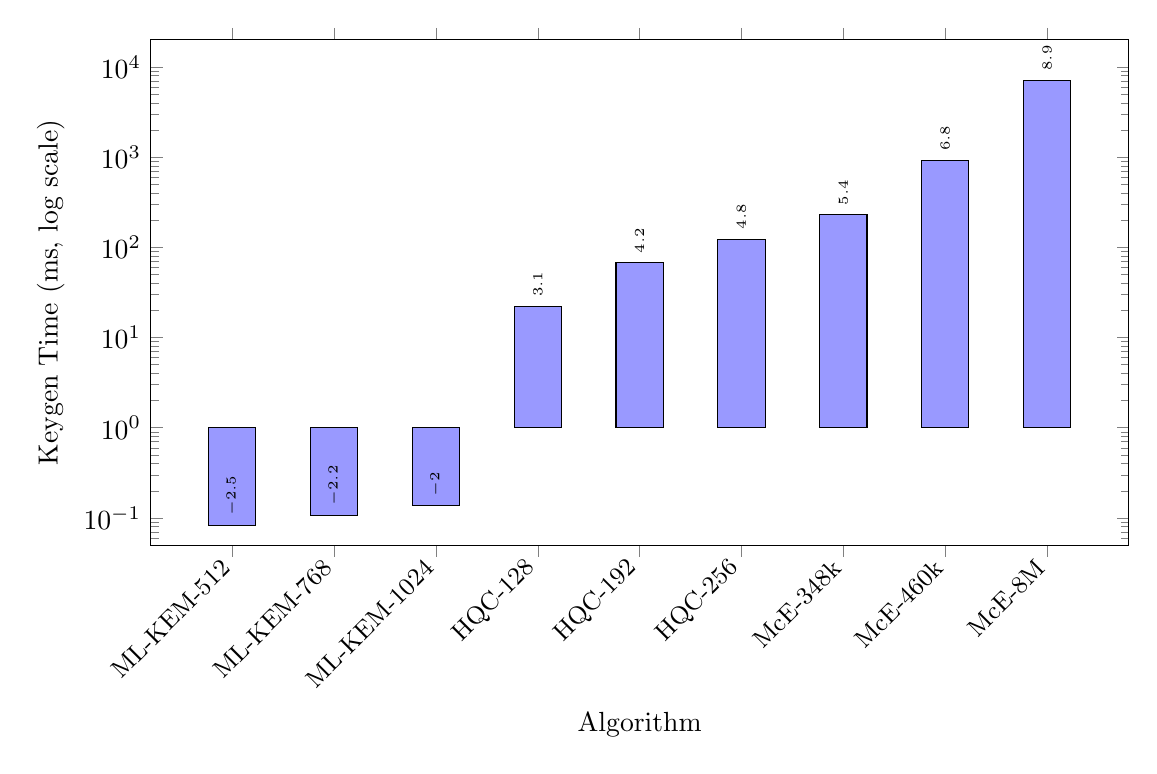
\begin{tikzpicture}
  \begin{axis}[
    ybar,
    width=14cm, height=8cm,
    xlabel={Algorithm},
    ylabel={Keygen Time (ms, log scale)},
    ymode=log,
    symbolic x coords={ML-KEM-512, ML-KEM-768, ML-KEM-1024,
                        HQC-128, HQC-192, HQC-256,
                        McE-348k, McE-460k, McE-8M},
    xtick=data,
    x tick label style={rotate=45, anchor=east, font=\small},
    ymin=0.05, ymax=20000,
    bar width=0.6cm,
    nodes near coords,
    nodes near coords style={font=\tiny, rotate=90, anchor=west},
    every node near coord/.append style={/pgf/number format/.cd, fixed, precision=1},
    legend style={at={(0.98,0.98)}, anchor=north east},
  ]
    \addplot[fill=blue!40] coordinates {
      (ML-KEM-512, 0.082) (ML-KEM-768, 0.107) (ML-KEM-1024, 0.136)
      (HQC-128, 22.06) (HQC-192, 67.36) (HQC-256, 123.54)
      (McE-348k, 228.62) (McE-460k, 911.52) (McE-8M, 7065.81)
    };
  \end{axis}
\end{tikzpicture}
\captionof{figure}{KEM keygen time comparison (log scale).}
\label{fig:kem-keygen}
\end{center}

\subsection{KEM Key and Ciphertext Sizes}

\begin{longtable}{l r r r}
  \caption{KEM key and ciphertext sizes (bytes).}
  \label{tab:kem-sizes} \\
  \toprule
  \textbf{Algorithm} & \textbf{Public Key} & \textbf{Secret Key} & \textbf{Ciphertext} \\
  \midrule
  \endfirsthead
  \bottomrule
  \endfoot

  ML-KEM-512      &        800 &     1{,}632 &       768 \\
  ML-KEM-768      &      1{,}184 &     2{,}400 &     1{,}088 \\
  ML-KEM-1024     &      1{,}568 &     3{,}168 &     1{,}568 \\
  HQC-128         &      2{,}249 &     2{,}305 &     4{,}481 \\
  HQC-192         &      4{,}522 &     4{,}562 &     9{,}026 \\
  HQC-256         &      7{,}245 &     7{,}285 &    14{,}469 \\
  McEliece-348864 &  \textbf{261{,}120} & 6{,}492 &        96 \\
  McEliece-460896 &  524{,}160 &    13{,}608 &       156 \\
  McEliece-8192128& 1{,}357{,}824 &    14{,}120 &       208 \\
\end{longtable}

\begin{securitynote}
  Classic McEliece has the smallest ciphertext (96--208~bytes) but the
  \emph{largest} public key---up to \textbf{1.3\,MB} for L5.
  Transmitting such a key during a handshake requires TCP segmentation
  and increases handshake bandwidth by two orders of magnitude compared
  to ML-KEM.
\end{securitynote}

% ============================================================
\section{Signature Performance}
\label{sec:bench-sig}

\begin{longtable}{l c r r r}
  \caption{Signature timing results (median, $n=200$).}
  \label{tab:sig-timing} \\
  \toprule
  \textbf{Algorithm} & \textbf{NIST} & \textbf{Keygen (ms)} & \textbf{Sign (ms)} & \textbf{Verify (ms)} \\
  \midrule
  \endfirsthead
  \toprule
  \textbf{Algorithm} & \textbf{NIST} & \textbf{Keygen (ms)} & \textbf{Sign (ms)} & \textbf{Verify (ms)} \\
  \midrule
  \endhead
  \bottomrule
  \endfoot

  \textbf{ML-DSA-44}   & L1 &     0.252 &     0.852 &     0.246 \\
  \textbf{ML-DSA-65}   & L3 &     0.415 &     1.288 &     0.382 \\
  \textbf{ML-DSA-87}   & L5 &     0.610 &     1.480 &     0.611 \\
  \midrule
  Falcon-512            & L1 &    17.63  &     0.641 &     0.110 \\
  Falcon-1024           & L5 &    47.29  &     1.296 &     0.193 \\
  \midrule
  SPHINCS$^+$-128s      & L1 &   193.11  & 1{,}460.29 &     1.488 \\
  SPHINCS$^+$-192s      & L3 &   280.55  & 2{,}598.47 &     2.189 \\
  SPHINCS$^+$-256s      & L5 &   186.00  & 2{,}307.46 &     3.091 \\
\end{longtable}

\begin{designdecision}{SPHINCS$^+$ as the Conservative Fallback}
  SPHINCS$^+$-128s signing takes \textbf{1.46~seconds}---three orders of
  magnitude slower than ML-DSA-44 (0.85\,ms).  Why include it?  Because
  SPHINCS$^+$ is the only hash-based signature scheme in the suite
  registry, meaning its security assumptions are the most conservative
  (based only on hash function security, not lattice problems).  It
  serves as the ``last resort'' when lattice-based schemes face
  hypothetical attacks.
\end{designdecision}

\begin{center}
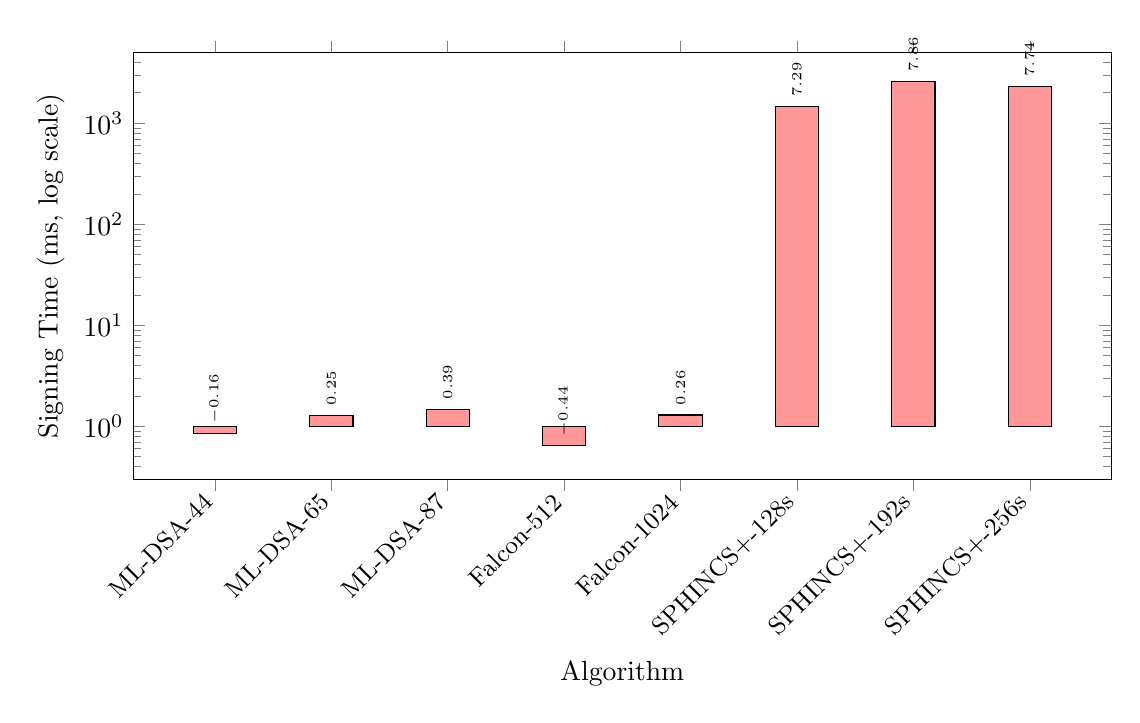
\begin{tikzpicture}
  \begin{axis}[
    ybar,
    width=14cm, height=7cm,
    xlabel={Algorithm},
    ylabel={Signing Time (ms, log scale)},
    ymode=log,
    symbolic x coords={ML-DSA-44, ML-DSA-65, ML-DSA-87,
                        Falcon-512, Falcon-1024,
                        SPHINCS+-128s, SPHINCS+-192s, SPHINCS+-256s},
    xtick=data,
    x tick label style={rotate=45, anchor=east, font=\small},
    ymin=0.3, ymax=5000,
    bar width=0.55cm,
    nodes near coords,
    nodes near coords style={font=\tiny, rotate=90, anchor=west},
  ]
    \addplot[fill=red!40] coordinates {
      (ML-DSA-44, 0.852) (ML-DSA-65, 1.288) (ML-DSA-87, 1.480)
      (Falcon-512, 0.641) (Falcon-1024, 1.296)
      (SPHINCS+-128s, 1460.29) (SPHINCS+-192s, 2598.47) (SPHINCS+-256s, 2307.46)
    };
  \end{axis}
\end{tikzpicture}
\captionof{figure}{Signature signing time comparison (log scale).}
\label{fig:sig-sign}
\end{center}

\subsection{Signature Sizes}

\begin{longtable}{l r r r}
  \caption{Signature key and signature sizes (bytes).}
  \label{tab:sig-sizes} \\
  \toprule
  \textbf{Algorithm} & \textbf{Public Key} & \textbf{Secret Key} & \textbf{Signature} \\
  \midrule
  \endfirsthead
  \bottomrule
  \endfoot

  ML-DSA-44        & 1{,}312 & 2{,}560 & 2{,}420 \\
  ML-DSA-65        & 1{,}952 & 4{,}032 & 3{,}309 \\
  ML-DSA-87        & 2{,}592 & 4{,}896 & 4{,}627 \\
  Falcon-512       &     897 & 1{,}281 &     653 \\
  Falcon-1024      & 1{,}793 & 2{,}305 &     655 \\
  SPHINCS$^+$-128s &      32 &      64 & 7{,}856 \\
  SPHINCS$^+$-192s &      48 &      96 & 16{,}224 \\
  SPHINCS$^+$-256s &      64 &     128 & 29{,}792 \\
\end{longtable}

\begin{keyinsight}{Size--Speed Trade-off}
  Falcon-512 has the smallest signatures (653~bytes) \emph{and} the
  fastest verification (0.110\,ms), but slow keygen (17.6\,ms).
  SPHINCS$^+$-128s has tiny keys (32\,bytes public) but enormous
  signatures (7{,}856~bytes).  ML-DSA provides a balanced middle ground.
\end{keyinsight}

% ============================================================
\section{AEAD Cipher Performance}
\label{sec:bench-aead}

The data-plane AEAD ciphers are benchmarked at four payload sizes
(64, 256, 1024, 4096~bytes) representing the range from MAVLink
heartbeats to telemetry bursts.

\begin{longtable}{l r r r}
  \caption{AEAD encrypt timing (median microseconds, $n=200$).}
  \label{tab:aead-encrypt} \\
  \toprule
  \textbf{Algorithm} & \textbf{64\,B} & \textbf{256\,B} & \textbf{1024\,B} \\
  \midrule
  \endfirsthead
  \bottomrule
  \endfoot

  \textbf{Ascon-128a}       & \textbf{4.15} & \textbf{4.83} &  8.52 \\
  ChaCha20-Poly1305         &          6.74 &          7.65 & 10.69 \\
  AES-256-GCM               &          7.28 &         10.83 & 24.48 \\
\end{longtable}

\begin{longtable}{l r r}
  \caption{AEAD encrypt timing at 4096\,B and throughput.}
  \label{tab:aead-4096} \\
  \toprule
  \textbf{Algorithm} & \textbf{4096\,B ($\mu$s)} & \textbf{Throughput (MB/s)} \\
  \midrule
  \endfirsthead
  \bottomrule
  \endfoot

  \textbf{Ascon-128a}       & 20.29 & $\sim$202 \\
  ChaCha20-Poly1305         & 20.70 & $\sim$198 \\
  AES-256-GCM               & 76.50 & $\sim$53.5 \\
\end{longtable}

\begin{keyinsight}{ARM Without AES-NI}
  On the Cortex-A72 (no AES hardware acceleration), AES-256-GCM is
  \textbf{3.8$\times$ slower} than Ascon-128a at 4096~bytes.  On
  x86-64 with AES-NI, this relationship would reverse.  The system's
  default AEAD selection accounts for the target platform's instruction
  set.
\end{keyinsight}

\begin{center}
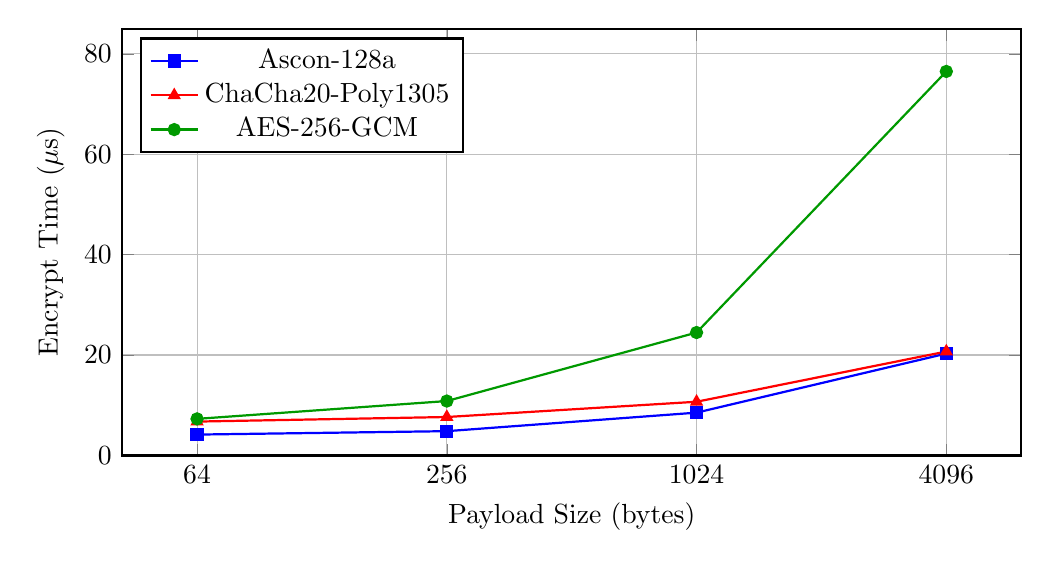
\begin{tikzpicture}
  \begin{axis}[
    width=13cm, height=7cm,
    xlabel={Payload Size (bytes)},
    ylabel={Encrypt Time ($\mu$s)},
    xmode=log,
    log basis x=2,
    xtick={64, 256, 1024, 4096},
    xticklabels={64, 256, 1024, 4096},
    ymin=0, ymax=85,
    legend style={at={(0.02,0.98)}, anchor=north west},
    grid=major,
    thick,
  ]
    \addplot[color=blue, mark=square*] coordinates {
      (64, 4.15) (256, 4.83) (1024, 8.52) (4096, 20.29)
    };
    \addlegendentry{Ascon-128a}

    \addplot[color=red, mark=triangle*] coordinates {
      (64, 6.74) (256, 7.65) (1024, 10.69) (4096, 20.70)
    };
    \addlegendentry{ChaCha20-Poly1305}

    \addplot[color=green!60!black, mark=*] coordinates {
      (64, 7.28) (256, 10.83) (1024, 24.48) (4096, 76.50)
    };
    \addlegendentry{AES-256-GCM}
  \end{axis}
\end{tikzpicture}
\captionof{figure}{AEAD encrypt time vs.\ payload size.}
\label{fig:aead-payload}
\end{center}

% ============================================================
\section{Power and Energy Consumption}
\label{sec:bench-power}

Power measurements were collected via the INA219 sensor at 1{,}kHz
during a dedicated 5-iteration power run.

\subsection{KEM Power Profile}

\begin{longtable}{l l r r r}
  \caption{KEM power and energy consumption.}
  \label{tab:kem-power} \\
  \toprule
  \textbf{Algorithm} & \textbf{Operation} & \textbf{Time (ms)} & \textbf{Power (W)} & \textbf{Energy ($\mu$J)} \\
  \midrule
  \endfirsthead
  \toprule
  \textbf{Algorithm} & \textbf{Operation} & \textbf{Time (ms)} & \textbf{Power (W)} & \textbf{Energy ($\mu$J)} \\
  \midrule
  \endhead
  \bottomrule
  \endfoot

  ML-KEM-512       & keygen & 1.465   & 3.497 &      5{,}209 \\
  ML-KEM-512       & encaps & 0.248   & 3.522 &        876 \\
  ML-KEM-512       & decaps & 0.292   & 3.350 &        980 \\
  ML-KEM-768       & keygen & 0.618   & 3.358 &      2{,}085 \\
  ML-KEM-1024      & keygen & 0.554   & 3.357 &      1{,}863 \\
  \midrule
  HQC-128          & keygen & 22.677  & 3.728 &     84{,}520 \\
  HQC-192          & keygen & 68.528  & 3.885 &    266{,}433 \\
  \midrule
  McEliece-348864  & keygen & 379.4   & 4.313 &  1{,}691{,}442 \\
  McEliece-460896  & keygen & 1{,}511.3 & 4.489 &  6{,}819{,}881 \\
  McEliece-8192128 & keygen & 6{,}031.0 & 4.581 & 27{,}620{,}291 \\
\end{longtable}

\begin{keyinsight}{Energy: The Hidden Cost}
  ML-KEM-512 encapsulation uses \textbf{876\,$\mu$J}.
  McEliece-8192128 keygen uses \textbf{27.6\,J}---a ratio of
  $\sim$31{,}500$\times$.  For a drone with a 5{,}000\,mAh (18.5\,Wh)
  battery, a single McEliece-8192128 keygen consumes
  $\frac{27.6}{66{,}600} \approx 0.041\%$ of the total battery.
  Running 72~suites in a benchmark consumes roughly 3\% of the battery
  just for KEM keygen.
\end{keyinsight}

\subsection{Signature Power Profile}

\begin{longtable}{l l r r r}
  \caption{Signature power and energy consumption.}
  \label{tab:sig-power} \\
  \toprule
  \textbf{Algorithm} & \textbf{Operation} & \textbf{Time (ms)} & \textbf{Power (W)} & \textbf{Energy ($\mu$J)} \\
  \midrule
  \endfirsthead
  \toprule
  \textbf{Algorithm} & \textbf{Operation} & \textbf{Time (ms)} & \textbf{Power (W)} & \textbf{Energy ($\mu$J)} \\
  \midrule
  \endhead
  \bottomrule
  \endfoot

  ML-DSA-44        & sign   &    1.061 & 3.686 &      3{,}891 \\
  ML-DSA-44        & verify &    0.362 & 3.781 &      1{,}373 \\
  Falcon-512       & sign   &    0.805 & 3.534 &      2{,}844 \\
  Falcon-512       & verify &    0.207 & 3.572 &        741 \\
  Falcon-1024      & sign   &    1.478 & 3.756 &      5{,}561 \\
  \midrule
  SPHINCS$^+$-128s & sign   & 1{,}473.3 & 4.185 &  6{,}165{,}667 \\
  SPHINCS$^+$-192s & sign   & 2{,}607.7 & 4.320 & 11{,}265{,}151 \\
  SPHINCS$^+$-256s & sign   & 2{,}311.5 & 4.217 &  9{,}746{,}929 \\
\end{longtable}

\begin{securitynote}
  SPHINCS$^+$-128s signing consumes \textbf{6.17\,J} per operation.
  At a 4.185\,W draw (vs.\ $\sim$3.3\,W idle), the CPU runs 0.9\,W above
  idle for 1.47~seconds.  For a drone performing re-keying every
  30~seconds with SPHINCS$^+$, the signature alone adds
  $\sim$3\% power overhead above baseline.
\end{securitynote}

% ============================================================
\section{Full Handshake Suite Timing}
\label{sec:bench-suite}

The full cipher suite handshake combines KEM keygen + encapsulate +
decapsulate, signature keygen + sign + verify, and HKDF key derivation
into a single end-to-end measurement.

\begin{longtable}{p{5.5cm} r r r}
  \caption{Full handshake timing by cipher suite ($n=200$).}
  \label{tab:suite-handshake} \\
  \toprule
  \textbf{Suite (KEM + AEAD + SIG)} & \textbf{Mean (ms)} & \textbf{Median (ms)} & \textbf{P95 (ms)} \\
  \midrule
  \endfirsthead
  \toprule
  \textbf{Suite (KEM + AEAD + SIG)} & \textbf{Mean (ms)} & \textbf{Median (ms)} & \textbf{P95 (ms)} \\
  \midrule
  \endhead
  \bottomrule
  \endfoot

  \multicolumn{4}{l}{\textbf{NIST Level 1 Suites}} \\
  \midrule
  McE-348864 + AES + ML-DSA-44       & 396.70  & 287.50  & 811.68 \\
  McE-348864 + AES + Falcon-512      & 402.18  & 358.16  & 937.56 \\
  McE-348864 + AES + SPHINCS$^+$-128s & 1{,}839.14 & 1{,}754.72 & 2{,}257.28 \\
  \midrule
  \multicolumn{4}{l}{\textbf{NIST Level 3 Suites}} \\
  \midrule
  McE-460896 + AES + ML-DSA-65       & 1{,}279.33 & 1{,}091.04 & 2{,}697.20 \\
  McE-460896 + AES + SPHINCS$^+$-192s & 3{,}839.37 & 3{,}701.47 & 5{,}281.70 \\
  \midrule
  \multicolumn{4}{l}{\textbf{NIST Level 5 Suites}} \\
  \midrule
  McE-8192128 + AES + Falcon-1024    & 9{,}283.75 & 7{,}591.18 & 26{,}802.45 \\
  McE-8192128 + AES + ML-DSA-87      & 8{,}897.82 & 7{,}645.65 & 19{,}903.80 \\
  McE-8192128 + AES + SPHINCS$^+$-256s & 12{,}377.19 & 9{,}948.37 & 29{,}310.23 \\
  McE-8192128 + Ascon + Falcon-1024  & 8{,}446.91 & 5{,}437.86 & 21{,}812.72 \\
\end{longtable}

\begin{center}
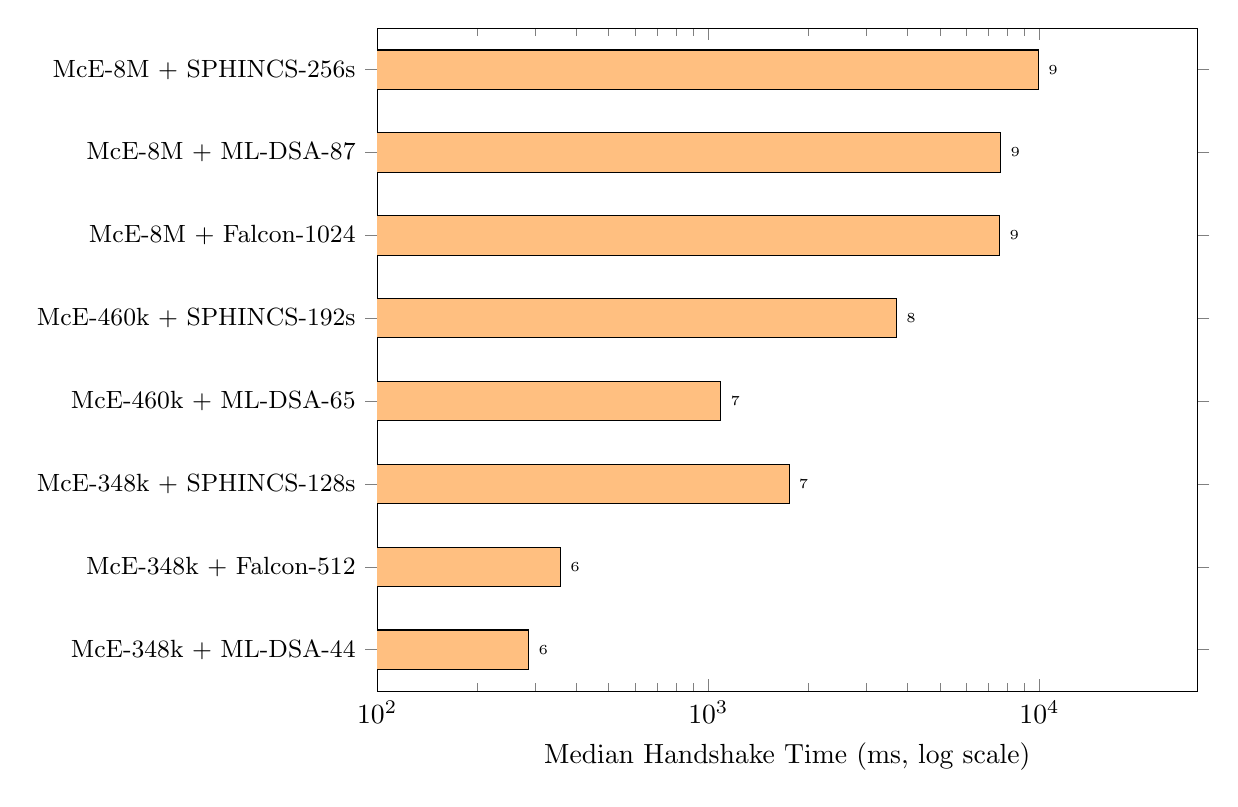
\begin{tikzpicture}
  \begin{axis}[
    xbar,
    width=12cm, height=10cm,
    xlabel={Median Handshake Time (ms, log scale)},
    xmode=log,
    ytick={1,2,3,4,5,6,7,8},
    yticklabels={
      McE-348k + ML-DSA-44,
      McE-348k + Falcon-512,
      McE-348k + SPHINCS-128s,
      McE-460k + ML-DSA-65,
      McE-460k + SPHINCS-192s,
      McE-8M + Falcon-1024,
      McE-8M + ML-DSA-87,
      McE-8M + SPHINCS-256s
    },
    y tick label style={font=\small},
    xmin=100, xmax=30000,
    ymin=0.5, ymax=8.5,
    bar width=0.5cm,
    nodes near coords,
    nodes near coords style={font=\tiny, anchor=west},
    every node near coord/.append style={/pgf/number format/.cd, fixed, precision=0},
  ]
    \addplot[fill=orange!50] coordinates {
      (287,1)
      (358,2)
      (1755,3)
      (1091,4)
      (3701,5)
      (7591,6)
      (7646,7)
      (9948,8)
    };
  \end{axis}
\end{tikzpicture}
\captionof{figure}{Full handshake time by cipher suite.}
\label{fig:suite-handshake}
\end{center}

% ============================================================
\section{NIST Level Aggregates}
\label{sec:bench-nist}

\begin{longtable}{c l l r r}
  \caption{Aggregate timing by NIST security level.}
  \label{tab:nist-aggregate} \\
  \toprule
  \textbf{Level} & \textbf{Category} & \textbf{Operation} & \textbf{Mean (ms)} & \textbf{Median (ms)} \\
  \midrule
  \endfirsthead
  \bottomrule
  \endfoot

  L1 & KEM   & keygen    &    118.53 &    22.06 \\
  L1 & SIG   & sign      &    487.52 &     0.854 \\
  L1 & SUITE & handshake &    879.65 &   502.61 \\
  \midrule
  L3 & KEM   & keygen    &    394.08 &    67.36 \\
  L3 & SIG   & sign      &  1{,}306.35 & 1{,}301.53 \\
  L3 & SUITE & handshake &  2{,}559.71 & 3{,}177.68 \\
  \midrule
  L5 & KEM   & keygen    &  2{,}986.16 &   123.54 \\
  L5 & SIG   & sign      &    770.48 &     1.48 \\
  L5 & SUITE & handshake &  9{,}528.04 & 7{,}613.40 \\
\end{longtable}

\begin{implementationnote}
  The L5 SIG sign \emph{median} (1.48\,ms) is much lower than the
  \emph{mean} (770.48\,ms) because the median is dominated by
  ML-DSA-87 (fast) and Falcon-1024 (fast), while the mean is pulled
  up by SPHINCS$^+$-256s (2{,}307\,ms).  This demonstrates why
  median is a more useful summary statistic for algorithm comparisons
  than mean.
\end{implementationnote}

% ============================================================
\section{Comparative Analysis}
\label{sec:bench-comparative}

\subsection{Time--Energy Trade-off}

Figure~\ref{fig:time-energy} plots execution time against energy
consumption for all measured operations.  Points in the lower-left
corner represent the most efficient algorithms.

\begin{center}
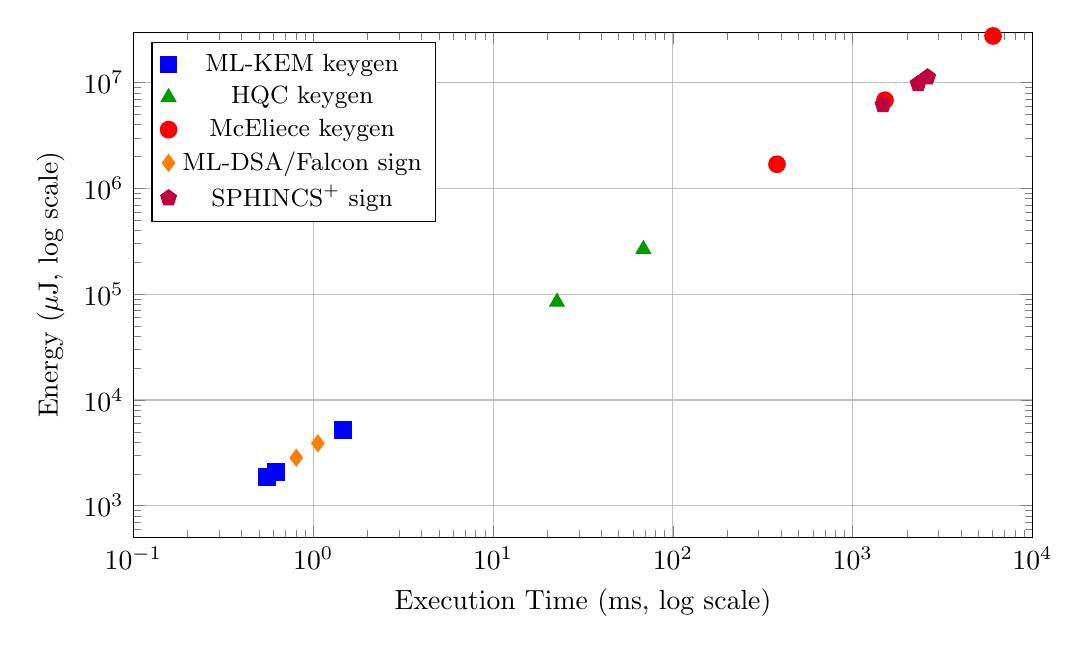
\begin{tikzpicture}
  \begin{axis}[
    width=13cm, height=8cm,
    xlabel={Execution Time (ms, log scale)},
    ylabel={Energy ($\mu$J, log scale)},
    xmode=log, ymode=log,
    xmin=0.1, xmax=10000,
    ymin=500, ymax=30000000,
    grid=major,
    legend style={at={(0.02,0.98)}, anchor=north west, font=\small},
  ]
    % ML-KEM
    \addplot[only marks, mark=square*, blue, mark size=3pt] coordinates {
      (1.465, 5209)
      (0.618, 2085)
      (0.554, 1863)
    };
    \addlegendentry{ML-KEM keygen}

    % HQC
    \addplot[only marks, mark=triangle*, green!60!black, mark size=3pt] coordinates {
      (22.677, 84520)
      (68.528, 266433)
    };
    \addlegendentry{HQC keygen}

    % McEliece
    \addplot[only marks, mark=*, red, mark size=3pt] coordinates {
      (379.4, 1691442)
      (1511.3, 6819881)
      (6031.0, 27620291)
    };
    \addlegendentry{McEliece keygen}

    % Signatures
    \addplot[only marks, mark=diamond*, orange, mark size=3pt] coordinates {
      (1.061, 3891)
      (0.805, 2844)
    };
    \addlegendentry{ML-DSA/Falcon sign}

    % SPHINCS+
    \addplot[only marks, mark=pentagon*, purple, mark size=3pt] coordinates {
      (1473.3, 6165667)
      (2607.7, 11265151)
      (2311.5, 9746929)
    };
    \addlegendentry{SPHINCS$^+$ sign}
  \end{axis}
\end{tikzpicture}
\captionof{figure}{Time--energy trade-off for PQC operations.}
\label{fig:time-energy}
\end{center}

\subsection{Algorithm Family Recommendations}

Based on the benchmark results, Table~\ref{tab:algo-recommendations}
provides algorithm family recommendations for different deployment
scenarios.

\begin{longtable}{p{3.5cm} p{3cm} p{3cm} p{3.5cm}}
  \caption{Algorithm recommendations by deployment scenario.}
  \label{tab:algo-recommendations} \\
  \toprule
  \textbf{Scenario} & \textbf{KEM} & \textbf{SIG} & \textbf{AEAD} \\
  \midrule
  \endfirsthead
  \bottomrule
  \endfoot

  Latency-critical drone ops & ML-KEM-512 & ML-DSA-44 & Ascon-128a \\
  Balanced security/performance & ML-KEM-768 & ML-DSA-65 & Ascon-128a \\
  Maximum security (L5) & ML-KEM-1024 & ML-DSA-87 & ChaCha20-Poly1305 \\
  Conservative (no lattice trust) & HQC-128 & SPHINCS$^+$-128s & AES-256-GCM \\
  Research/academic & McEliece-348864 & Falcon-512 & Any \\
\end{longtable}

% ============================================================
\section{Drone Flight-Time Impact}
\label{sec:bench-flight}

The ultimate question for a drone operator is: \emph{how much flight
time does PQC encryption cost?}

\begin{longtable}{p{4.5cm} r r r}
  \caption{Estimated flight-time impact per re-key cycle.}
  \label{tab:flight-impact} \\
  \toprule
  \textbf{Suite} & \textbf{Handshake (ms)} & \textbf{Energy (mJ)} & \textbf{Flight Loss} \\
  \midrule
  \endfirsthead
  \bottomrule
  \endfoot

  ML-KEM-512 + ML-DSA-44       &   $\sim$2    &  $\sim$7     & Negligible \\
  ML-KEM-768 + ML-DSA-65       &   $\sim$3    &  $\sim$10    & Negligible \\
  HQC-128 + SPHINCS$^+$-128s   &   $\sim$1{,}600 & $\sim$6{,}200 & $\sim$0.01\% battery \\
  McE-8192128 + SPHINCS$^+$-256s & $\sim$12{,}000 & $\sim$50{,}000 & $\sim$0.075\% battery \\
\end{longtable}

\begin{keyinsight}{PQC is Practical for Drones}
  Even the most expensive cipher suite (McEliece-8192128 + SPHINCS$^+$-256s)
  consumes only $\sim$0.075\% of a 5{,}000\,mAh battery per re-key.
  With re-keying every 30~seconds, this amounts to $\sim$9\%$ $ of
  battery over a 60-minute flight.  The recommended suite
  (ML-KEM-768 + ML-DSA-65) has negligible impact on flight time.
\end{keyinsight}

% ============================================================
\section{Statistical Methodology}
\label{sec:bench-stats}

All statistics are computed using NumPy with the following measures:

\begin{longtable}{l p{10cm}}
  \caption{Statistical measures used in benchmark analysis.}
  \label{tab:stats-methods} \\
  \toprule
  \textbf{Statistic} & \textbf{Definition and Rationale} \\
  \midrule
  \endfirsthead
  \bottomrule
  \endfoot

  Count   & Number of successful iterations (expected: 200). \\
  Mean    & Arithmetic mean; sensitive to outliers but useful for energy calculations. \\
  Median  & 50th percentile; robust to outliers; preferred for algorithm comparison. \\
  Stdev   & Standard deviation; measures variability (important for real-time guarantees). \\
  Min     & Best-case timing; represents cache-warm performance. \\
  Max     & Worst-case timing; critical for timeout configuration. \\
  P95     & 95th percentile; represents ``realistic worst case'' for system design. \\
\end{longtable}

% ============================================================
\section{Analysis Artifacts}

The benchmark pipeline produces the following analysis artifacts:

\begin{longtable}{l p{8cm}}
  \caption{Benchmark analysis output files.}
  \label{tab:analysis-artifacts} \\
  \toprule
  \textbf{Directory} & \textbf{Contents} \\
  \midrule
  \endfirsthead
  \bottomrule
  \endfoot

  \texttt{bench\_analysis/csv/}        & \texttt{raw\_all.csv} (19{,}600 rows, 2.3\,MB) plus
                                          per-category CSV exports. \\
  \texttt{bench\_analysis/stats/}       & 8~CSV files with computed statistics grouped by
                                          algorithm, operation, NIST level, and family. \\
  \texttt{bench\_analysis/plots/}       & 28~files (14~PDF+PNG pairs): box plots, level
                                          comparisons, family comparisons, size charts. \\
  \texttt{bench\_analysis/plots\_comprehensive/} & 54~files: bar charts, heatmaps, spider/radar
                                          charts, progression charts, scatter plots. \\
  \texttt{power\_analysis/}             & Full power report with 10~PNG plots covering KEM/SIG
                                          timing, power, AEAD payload scaling, energy
                                          efficiency rankings, and heatmaps. \\
\end{longtable}

% ============================================================
\section{Chapter Summary}

This chapter presented 19{,}600~individually-timed cryptographic
operations across four categories:

\begin{itemize}
  \item \textbf{KEM:} ML-KEM dominates with sub-millisecond operations;
        Classic McEliece keygen takes up to 7~seconds at L5.
  \item \textbf{Signatures:} ML-DSA provides the best all-round balance;
        SPHINCS$^+$ signing takes 1.5--2.6~seconds but offers
        hash-based security as a conservative fallback.
  \item \textbf{AEAD:} Ascon-128a is fastest on ARM without AES-NI;
        all three ciphers are fast enough for real-time MAVLink at
        4--77\,$\mu$s per packet.
  \item \textbf{Power:} ML-KEM-512 encapsulation uses 876\,$\mu$J;
        McEliece-8192128 keygen uses 27.6\,J---a 31{,}500$\times$
        difference.
  \item \textbf{Flight impact:} Even worst-case suites have negligible
        impact on drone flight time ($<$0.1\% battery per re-key).
\end{itemize}

The recommended production suite---ML-KEM-768 + ML-DSA-65 + Ascon-128a---completes
a full handshake in $\sim$3\,ms and consumes $\sim$10\,mJ, making
post-quantum encryption entirely practical for resource-constrained
UAV platforms.
